\chapter{Semi-spontaneous production}\label{sec:6}

\section{Research questions and rationale}\label{sec:07:1}

Following the analysis of learner performance in the structured tests, the present chapter aims to observe learners' morphosyntactic skills in a more realistic communicative situation, arguably closer to real language use. To this end, it presents and discusses the output elicited through a semi-spontaneous production task in which learners took part in pairs or small groups. Because of the amount of work required to transcribe and analyse such interactional data, only a subset of the database (the Italian Meaning Based edition of the project) will be considered.

After a qualitative analysis of learner-produced utterances, the study will apply the same statistical tool employed in the previous chapters in order to determine whether or not learners may be thought to apply a morphosyntactic principle in their output. The results are then compared to the scenarios identified in the previous chapters in order to appropriately collocate semi-spontaneous production along an implicational scale of task difficulty.

\section{An overview of learner output}\label{sec:07:2}

In learners' utterances, new referents are typically introduced by a copular construction with presentative function, in which the topic is expressed by a personal pronoun (\textit{on,} ‘he’ or \textit{ona}, ‘she’) and the complement is instantiated by the name of the character \REF{ex:07:1}.

\ea%1
    \label{ex:07:1}
    \ea\label{ex:07:1a}
    \gll    [ˈɔna   jɛst   ʤoˈvann-a].\\
            \hspaceThis{[}she  is  Giovanna-\textsc{nom}\\
    \glt    ‘She is Giovanna.’
    \ex\label{ex:07:1b}
    \gll    [ʤoˈvann-a     ɛst   nauʧiˈʧɛlk-on].  \\
            \hspaceThis{[}Giovanna-\textsc{nom}  is  teacher-\textsc{ins}\\
    \glt    ‘Giovanna is a teacher.’
    \z
\z

When a referent has been introduced, it is typically referred to using personal pronouns \REF{ex:07:2}, although person names may be repeated in consecutive utterances \REF{ex:07:3}:

\ea%2
    \label{ex:07:2}
    \ea\label{ex:07:2a}
    \gll    [to   jest   ˈmarj-a].\\
            \hspaceThis{[}this  is  Maria-\textsc{nom}\\
    \glt    ‘This is Maria.’
    \ex\label{ex:07:2b}
    \gll    [ˈɔna   ˈlubi   herˈbat-a].\\
            \hspaceThis{[}she  likes  tea-\textsc{nom}\\
    \glt    ‘She likes tea.’
    \z
\z

\ea%3
    \label{ex:07:3}
    \ea\label{ex:07:3a}
    \gll    [to   jest   ˈmarj-a].\\
            \hspaceThis{[}this  is  Maria-\textsc{nom}\\
    \glt    ‘This is Maria’
    \ex\label{ex:07:3b}
    \gll    [ˈmarj-a   jest   ˈnjemk-on  i   tuˈmaʧk-on].\\
            \hspaceThis{[}Maria-\textsc{nom}  is  German-\textsc{ins}  and  interpreter-\textsc{ins}\\
    \glt    ‘Maria is German and an interpreter.’
    \z
\z

Zero anaphora can be encountered \REF{ex:07:4b} following utterances in which the subject is expressed by either a name or a pronoun \REF{ex:07:4a}.

\ea%4
    \label{ex:07:4}
    \ea\label{ex:07:4a}
    \gll    [ˈɔna     jɛst   portuˈgalk-on (...)].\\
            \hspaceThis{[}she\textsc{.nom}  is  Portuguese-\textsc{ins}\\
    \glt    ‘She is Portuguese.’
    \ex\label{ex:07:4b}
    \gll    [i   zna   ˈjɛski         anˈgjelsk-i].\\
            \hspaceThis{[}and  knows  language\textsc{.nom/acc(?)}  English-\textsc{nom}/\textsc{acc} \\
    \glt    ‘And she speaks English.’
    \z
\z

No examples can be found in which common nouns express the subject function. 

Nouns in the object function may be correctly marked as accusative, both in a sequence of feminine nouns only \REF{ex:07:5a} and in sequences containing both feminine and masculine nouns  (\ref{ex:07:5b}, where \textit{kot} ‘cat’ and \textit{pies} ‘dog’ are masculine):

\ea%5
    \label{ex:07:5}
    \ea{\label{ex:07:5a}
    \gll    [ɔn   ˈlubi   ʧokoˈlad-e     ˈkav-e     i   erˈbat-e].\\
            \hspaceThis{[}He  likes  chocolate-\textsc{acc}    coffee-\textsc{acc}  and  tea-\textsc{acc}\\}\jambox*{(5106)}
    \glt    ‘He likes chocolate, coffee and tea.’
    \ex{\label{ex:07:5b}
    \gll    [ˈkɔxa  ˈʒɔn-e    ˈev-e    ˈkɔt-a    i  ps-a].\\
            \hspaceThis{[}loves  wife-\textsc{acc}  Ewa-\textsc{acc}   cat-\textsc{acc}    and  dog-\textsc{acc}\\}\jambox*{(5111)}
    \glt    ‘(He) loves his wife Ewa and (his) cat and (his) dog.’
    \z
\z

At the other end of the spectrum, occurrences can be found in which all feminine nouns in the object function are marked as nominative \REF{ex:07:6}:

\ea%6
    \label{ex:07:6}
    \ea{\label{ex:07:6a}
    \gll    [ˈɔna   ˈlubi   herˈbat-a].\\
            \hspaceThis{[}she  likes  tea-\textsc{nom}\\}\jambox*{(5119)}
    \glt    ‘She likes tea.’
    \ex{\label{ex:07:6b}
    \gll    [ˈɔna   ˈlubi   ʧekoˈlad-a     ˈkav-a     i   erˈbat-a].\\
            \hspaceThis{[}she  likes  chocolate-\textsc{nom}  coffee-\textsc{nom}  and  tea-\textsc{nom}\\}\jambox*{(5107)}
    \glt    ‘She likes chocolate, coffee and tea.’
    \z
\z

In other cases still, feminine nouns with the object function seem to randomly appear with a nominative or accusative endings, with no apparent regularity \REF{ex:07:7}:

\ea{%7
    \label{ex:07:7}
    \gll    {ˈɔna}   {ˈlubi}   {erˈbat-e}   {i}   {ˈkav-a.}\\
            she  likes  tea-\textsc{acc}  and  coffee-\textsc{nom}\\}\jambox*{(5107)}
    \glt    ‘She likes tea and coffee.’
    \z

Errors in the case marking of the object most commonly involve an overextension of the NOM ending -[a]. Marginal non-target-like endings include bare consonants and [ən], with 6 and 1 instances respectively (\tabref{tab:07:1}). In some cases the influence of other known languages can be hypothesised, as in [matemaˈtik] as opposed to German \textit{Mathematik} /matemaˈtiːk/. In other cases, the ending may be modelled on other word forms present in the input: in [kerbatən], for instance, the ending [ən] may be a trace of the instrumental masculine ending -\textit{em} -[em]. 

\begin{table}
    \begin{tabularx}{\textwidth}{llll}
        \lsptoprule
        learner & utterance & learner form & target\\
        \midrule
        5101 & [i ma dzurk]. & [dzurk] & /ˈtsurke/\\
        5118 & [ˈpaolo ˈlubi matemaˈtik i muˈzik]. & [matemaˈtik] & /mateˈmatɨke/\\
        5118 & [ˈpaolo ˈlubi matemaˈtik i muˈzik]. & [muˈzik] & /ˈmuzɨke/\\
        5115 & [on ˈlubi literaˈtura i mateˈmatik]. & [mateˈmatik] & /mateˈmatɨke/\\
        5117 & [ɔn ˈlubi mateˈmatik i psa]. & [mateˈmatik] & /mateˈmatɨke/\\
        5117 & [ˈmarta ˈlubi kav i kerˈbatən]. & [kav] & /ˈkave/\\
        5117 & [ˈmarta ˈlubi kav i kerˈbatən]. & [kerˈbatən] & /herˈbate/\\
        \lspbottomrule
    \end{tabularx}
    \caption{Semi-spontaneous production task, endings other than -/a/ or -/e/}
    \label{tab:07:1}
\end{table}

As such non-target endings were produced by only four learners, it seems that this phenomenon should be a matter of individual variability whose causes are beyond experimental control. 

No examples of OS word order were found in the data. 

\subsection{Morphological variability and relation to the input}\label{sec:07:2.1}

The present section aims to describe morphological variability among the lexemes which occur in the OBJ function. The purpose of this step is to verify whether or not the semantics of specific lexical items associates them more closely to either syntactic function (as indeed is the case in the input, see \chapref{sec:3}) and consequently to a specific inflectional ending.

To this purpose, \tabref{tab:07:2} lists the lexemes produced by learners along with their English translation. For each entry, the table indicates first the citation form and its English translation, then the overall accuracy with which the word received accusative marking (“mean"). This value is computed as the ratio between the number of accusative forms and the total number of occurrences (“freq") produced by all participants in contexts expressing the Object function. The following column (“participants”) indicates the number of participants who produced the lexeme (regardless of how it was inflected). The last four columns provide the frequency with which the word occurred in the input at the time of the test, i.e. after 10:30 hours. Figures are presented relatively to the NOM and ACC cases as well as cumulatively for all other cases combined (“other"). Given the nature of the task, not many occurrences were elicited for each lexeme: the most common item (\textit{literatura}, ‘literature’) occurred 17 times in the whole dataset, while 6 words (e.g. \textit{rodzina}, ‘family’) only occurred once. 

\begin{table}
    \fittable{
    \begin{tabular}{ll rrr  rrrr}
        \lsptoprule
         &  & \multicolumn{3}{c}{output} & \multicolumn{4}{c}{input}\\
         \cmidrule(r){3-5}\cmidrule(l){6-9}
        lexeme & translation & Mean & Freq. & participants & NOM & ACC & other & Tot\\
        \midrule
        \textit{Chorwacja} & Croatia & 1.00 & 2 & 1 & 1 & 0 & 2 & 3\\
        \textit{Ewa} & Ewa & 1.00 & 2 & 1 & 123 & 4 & 34 & 161\\
        \textit{rodzina} & family & 1.00 & 1 & 1 & 32 & 0 & 12 & 44\\
        \textit{tata} & dad & 1.00 & 1 & 1 & 54 & 19 & 0 & 73\\
        \textit{żona} & wife & 1.00 & 2 & 1 & 44 & 4 & 0 & 48\\
        \textit{herbata} & tea & 0.78 & 9 & 9 & 16 & 52 & 0 & 68\\
        \textit{kuchnia} & cuisine/kitchen & 0.75 & 4 & 3 & 20 & 22 & 0 & 42\\
        \textit{literatura} & literature & 0.71 & 17 & 11 & 1 & 53 & 0 & 54\\
        \textit{matematyka} & math & 0.57 & 7 & 5 & 0 & 9 & 0 & 9\\
        \textit{kola} & coke & 0.50 & 2 & 2 & 8 & 30 & 0 & 38\\
        \textit{mama} & mum & 0.50 & 2 & 1 & 54 & 8 & 0 & 62\\
        \textit{żaba} & frog & 0.50 & 2 & 2 & 61 & 48 & 0 & 109\\
        \textit{piłka} & ball & 0.33 & 3 & 3 & 30 & 23 & 0 & 53\\
        \textit{czekolada} & chocolate & 0.30 & 10 & 6 & 13 & 58 & 0 & 71\\
        \textit{kawa} & coffee & 0.30 & 10 & 6 & 36 & 48 & 0 & 84\\
        \textit{Anna} & Anna & 0.00 & 1 & 1 & 243 & 0 & 2 & 245\\
        \textit{córka} & daughter & 0.00 & 6 & 5 & 27 & 4 & 0 & 31\\
        \textit{lalka} & doll & 0.00 & 1 & 1 & 22 & 7 & 9 & 48\\
        \textit{muzyka} & music & 0.00 & 1 & 1 & 1 & 19 & 0 & 20\\
        \textit{pizza} & pizza & 0.00 & 1 & 1 & 12 & 31 & 0 & 43\\
        \textit{siostra} & sister & 0.00 & 3 & 2 & 19 & 13 & 3 & 45\\
        \lspbottomrule
    \end{tabular}
    }
    \caption{Lexemes produced by learners in interaction}
    \label{tab:07:2}
\end{table}

The following analysis is limited to common nouns, which leads to the exclusion of the names \textit{Anna,} \textit{Ewa} and \textit{Chorwacja}, ‘Croatia’. The rationale for this decision is that proper names may not be treated as common nouns, despite the fact that, in Polish, they are inflected  along the same inflectional paradigm. 

A certain degree of variability can also be found in the overall input frequency of the items considered here, the two extremes of the continuum being \textit{matematyka}, ‘mathematics’, with just 9 occurrences, and \textit{żaba}, ‘frog’, with 109. 

Regarding morphosyntactic accuracy, the whole continuum from 100\% to 0\% is represented. As made clear by example \REF{ex:07:7} above, different nouns may receive either marking even within the same utterance. 

It may be hypothesised that this variability in morphosyntactic accuracy may result from a biased distribution in the input: if a given lexeme mostly occurs in a specific word-form, then learners may associate it with the corresponding syntactic function or, at least, with the corresponding case marking. To exemplify, if a word only occurs in the accusative case, like \textit{matematyka,} ‘mathematics’, learners may note and remember it in its accusative form only. If this is the case, then accuracy for accusative case marking should be very high, in principle 100\%. In addition, this word-form should overextend to all others, including the nominative case: in other words, the basic word-form of this lexical item should be modelled on the accusative case.

One way to explain the observed variability in the accuracy of ACC marking is to hypothesise that this might be influenced by the proportion of instances in which a given lexeme appears in that word-form in the input. The more commonly the word appears in the input as ACC as opposed to NOM, the more accurately it should be marked as ACC in learner output as well.

If this is the case, plotting the relative frequency of accusative forms against case-marking accuracy should result in a straight line with a positive slope. \figref{fig:07:1}, however, shows no apparent pattern, suggesting that the expectations are not borne out in the data. Several words which in the input hardly ever occur in the accusative case show a mean accuracy of 100\% (e.g. \textit{rodzina} ‘family’), while others, whose ACC word form is much more common, exhibit much lower accuracy scores (e.g. \textit{muzyka} ‘music’).

\begin{figure}
    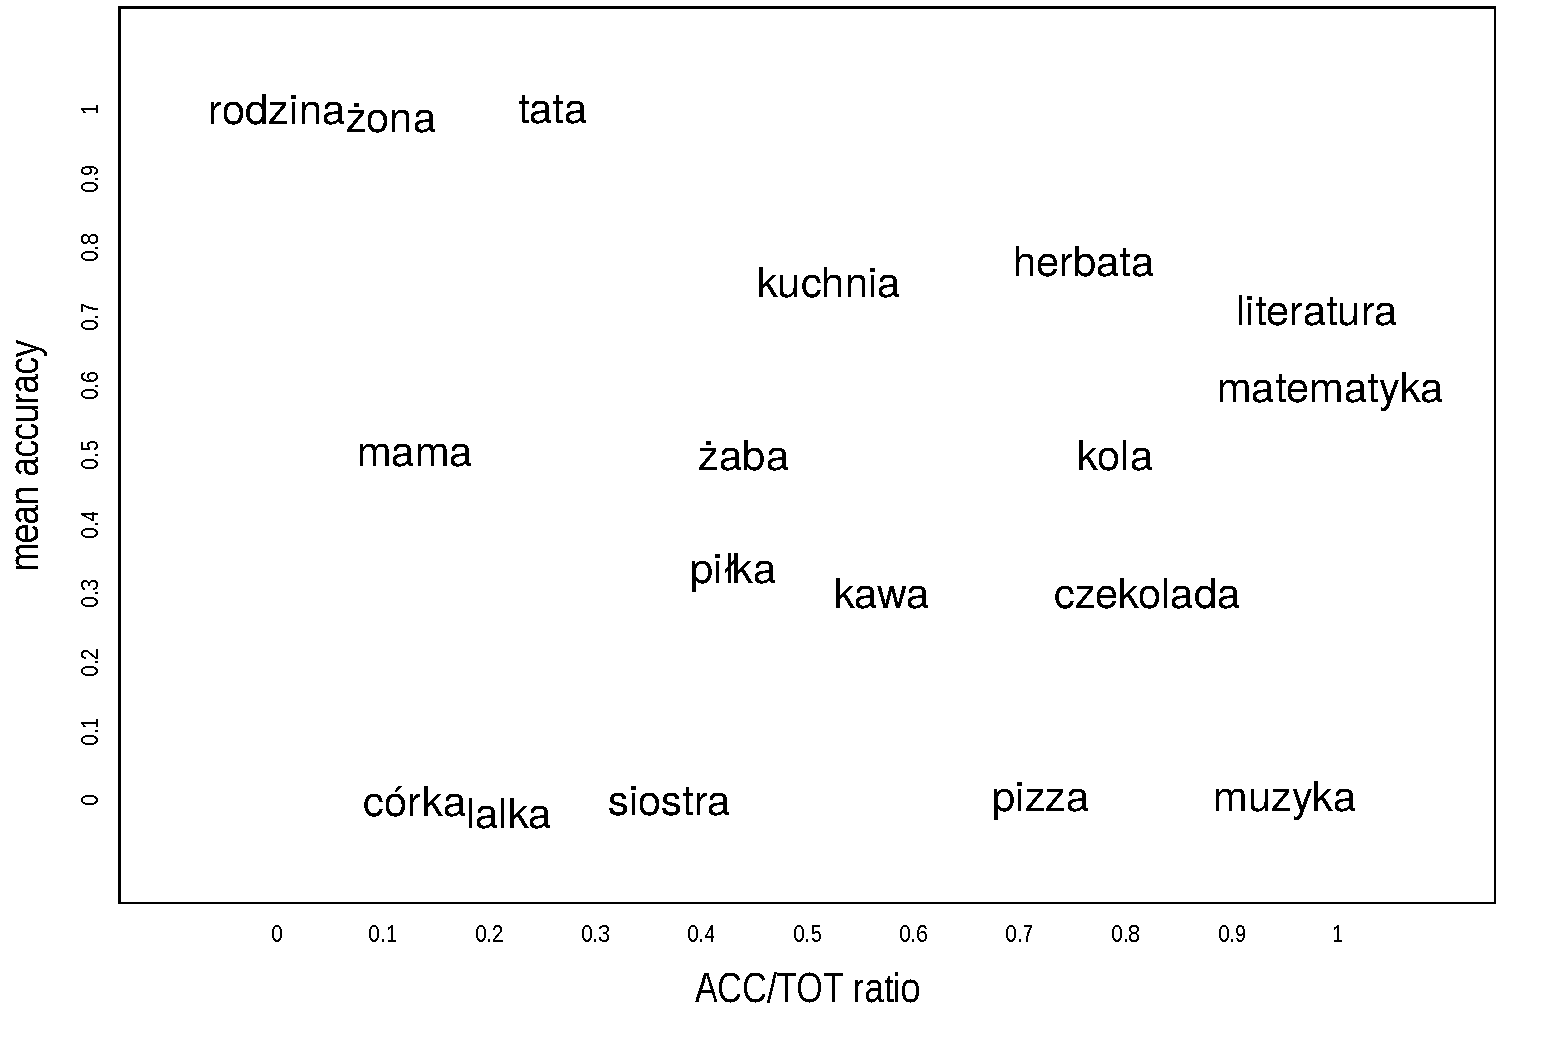
\includegraphics[width=\textwidth]{figures/07-1.pdf}
    \caption{Semi-spontaneous production, mean accuracy and ACC/TOT ratio}
    \label{fig:07:1}
\end{figure}

One may now consider the cumulative frequency of a given lexical item, in order to verify the claim that if a word is very frequent in the input, then it should be more available to the learners, and therefore more easily retrievable. In turn, if a word is easily retrievable, then perhaps the learner could devote more resources to inflectional morphology. 

If there were a correlation between overall lexical frequency and grammatical accuracy, lexemes in \figref{fig:07:2} should distribute along a positive slope, with accuracy increasing together with input frequency. Quite clearly, this is not the case. Differences in learners' morphosyntactic skills thus do not seem due to a biased distribution of word-forms in the input. 

\begin{figure}
    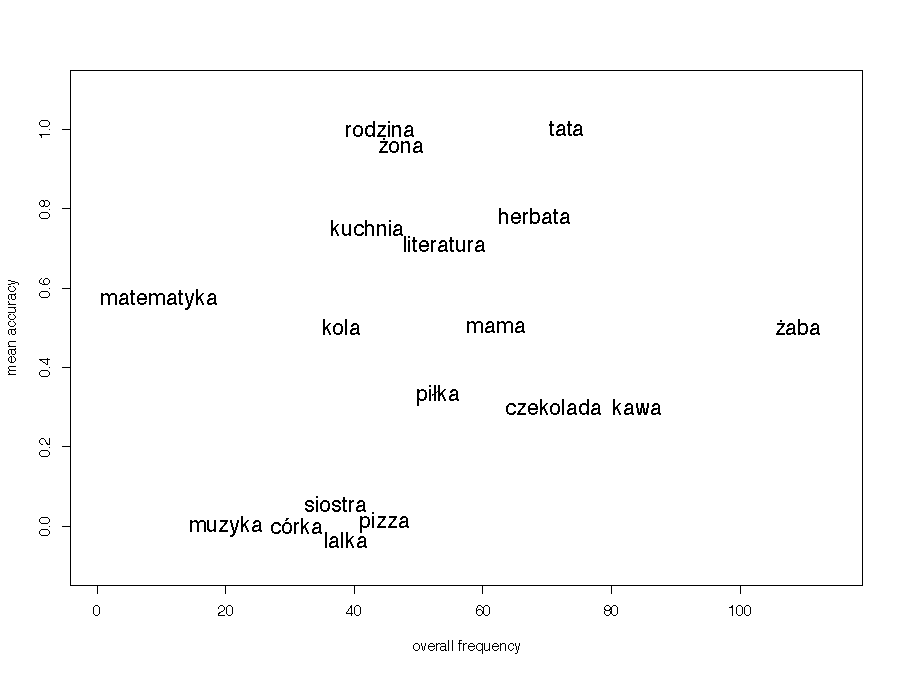
\includegraphics[width=\textwidth]{figures/07-2.pdf}
    \caption{Semi-spontaneous production task: mean accuracy / overall frequency}
    \label{fig:07:2}
\end{figure}

To conclude this section, it is worthwhile to point out that many of the words discussed in the analysis are fairly infrequent in the output data, as they were only produced by as few as a single learner. Tendencies regarding the properties of lexical items thus interact with the performance of individual learners, to which the next section is devoted. In any case, the analysis just concluded highlighted no obvious relation between input and output, in spite of the strong tendencies identified in the input (\chapref{sec:3}).

\subsection{Same-word utterances}\label{sec:07:2.2}

This section discusses case-marking variability within the same lexeme in the output of individual learners. The question may be pursued by looking at the output of participants with a mean accuracy different from 0 or 1, and in which the same lexical item occurs more than once (\tabref{tab:07:3}). If the rule governing case marking is simply unstable, then repeated lexical items should appear sometimes in their nominative, sometimes in their accusative form, with no apparent logic. If, on the other hand, case marking obeys a systematic principle, then each item should always appear in the same word-form in the same syntactic context.

\begin{table}
    \fittable{
    \begin{tabular}{lll}
        \lsptoprule
        participant & utterance & Lexeme\\
        \midrule
        5102 & [i ˈɔna ˈlubi literaˈture]. & [literaˈture]\\
        5102 & [i ɔn ˈlubi mateˈmatike literaˈture]. & [literaˈture; mateˈmatike]\\
        5102 & [i lubi mateˈmatike]. & [mateˈmatike]\\
        5102 & [i ˈkɔxa ˈʒɔne ˈeve i ˈkɔta i ˈkɔta i psa]. & [ˈʒɔne; ˈeve]\\
        5102 & [i ɔn ma ˈʒɔne ˈeve]. & [ˈʒɔne; ˈeve]\\
        5104 & [on ma ˈkɔta i sən i ˈtsurka]. & [ˈtsurka]\\
        5104 & [ɔn ma sən i ˈtsurka i forˈtɛpjan]. & [ˈtsurka]\\
        5109 & [ˈɔna ˈlubi ˈkava ərˈbate leteraˈtura]. & [ˈkava; ərˈbate; leteraˈtura]\\
        5109 & [on ˈlubi literaˈtura i mateˈmatike]. & [literaˈtura; mateˈmatike]\\
        5109 & [ɔn lu ɔn ˈlubi literaˈture mateˈmatike]. & [literaˈtura; mateˈmatike]\\
        5109 & [ˈɔna ˈlubi ˈkava i korˈvate ʧekoˈlada]. & [ˈkava; korˈvate; ʧekoˈlada]\\
        5109 & [ɔn ˈlubi ˈlɔde ʧekoˈlada i korˈvatje]. & [ʧekoˈlada; korˈvatj]e\\
        5113 & [ˈɔna ˈlubi literaˈtura ˈkave i i kɔt]. & [literaˈtura; ˈkave]\\
        5113 & [i ˈlubi literaˈtura i ˈkino i kerˈbate i ˈkava i psa i kot]. & [literaˈtura; kerˈbate; ˈkava]\\
        5115 & [krisˈtina ˈxoxa ˈmama ˈmame]. & [ˈmama ˈmame]\\
        \lspbottomrule
    \end{tabular}
    }
    \caption{Same-word utterances}
    \label{tab:07:3}
\end{table}

A few cases (e.g. the single utterance of learner 5115) are evident instances of disfluencies and self-corrections. Other learners exhibit a more variable picture of case-marking with the same lexical items. 5109 produces three instances of \textit{literatur-a}, ‘literature-\textsc{nom}’, and one of \textit{literatur-ę}, ‘literature-\textsc{acc}’; 5113 produces one instance of \textit{kaw-a}, ‘coffee-\textsc{nom}’, and one of \textit{kaw-ę}, ‘coffee-\textsc{acc}{}'.

With only these three exceptions, all other lexical items always occur in the same word-form, which can be indifferently -/e/ ACC (in the speech of learner 5102) or, more commonly, -/a/ NOM. 

\section{Evaluating a syntactic principle of utterance organisation}\label{sec:07:3}

In the following section, the statistical tool introduced in \chapref{sec:3} will be applied to the production data discussed in this chapter in order to verify whether or not learners use inflectional morphology in a target-like and systematic manner, that is, following a morphosyntactic principle.

It is worthwhile to start with an overview of the dataset. \tabref{tab:07:4} reports the lexemes produced by each participant in the ACC form. Not all learners produced all lexemes: the number of participants producing each lexeme ranges from a minimum of 1 (e.g. \textit{żona,} ‘wife’) to a maximum of 11 for \textit{literatura}, ‘literature’. 

\begin{table}
\fittable{
    \begin{tabular}{ll}
        \lsptoprule
                participant & lexemes\\
        \midrule
        5101 & \textit{czekolada,} \textit{kuchnia,} \textit{literatura,} \textit{siostra}\\
        5102 & \textit{córka,} \textit{Ewa,} \textit{literatura,} \textit{matematyka,} \textit{piłka,} \textit{siostra,} \textit{żaba,} \textit{żona}\\
        5104 & \textit{córka,} \textit{lalka,} \textit{literatura}\\
        5105 & \textit{Herbata}\\
        5106 & \textit{czekolada,} \textit{herbata,} \textit{kawa,} \textit{kola,} \textit{literatura}\\
        5107 & \textit{córka,} \textit{herbata,} \textit{kawa}\\
        5109 & \textit{chorwacja,} \textit{czekolada,} \textit{herbata,} \textit{kawa,} \textit{kuchnia,} \textit{literatura,} \textit{matematyka}\\
        5111 & \textit{herbata,} \textit{literatura}\\
        5112 & \textit{kuchnia,} \textit{literatura,} \textit{pizza} \\
        5113 & \textit{czekolada,} \textit{herbata,} \textit{kawa,} \textit{literatura,} \textit{żaba}\\
        5114 & \textit{Anna,} \textit{czekolada,} \textit{herbata,} \textit{kola,} \textit{piłka}\\
        5115 & \textit{córka,} \textit{literatura,} \textit{mama,} \textit{matematyka,} \textit{tata}\\
        5116 & \textit{literatura,} \textit{rodzina}\\
        5117 & \textit{herbata,} \textit{kawa,} \textit{literatura,} \textit{matematyka}\\
        5118 & \textit{córka,} \textit{matematyka,} \textit{muzyka}\\
        5119 & \textit{czekolada,} \textit{herbata,} \textit{kawa,} \textit{piłka}\\
        \lspbottomrule
    \end{tabular}
    }
    \caption{Lexemes produced by learners}
    \label{tab:07:4}
\end{table}

One can now proceed to verify what principle of utterance organisation each learner may be thought to have adopted. The analysis will only focus on those participants who produced at least three occurrences of a feminine noun in the object function. \tabref{tab:07:5} indicates the following information:
mean score (\textit{mean});
number of correctly case-marked feminine nouns (\textit{correct});
overall number of feminine nouns produced (\textit{contexts});
number of lexical types produced (\textit{lexemes});
ratio between number of utterances and number of lexical types, in which a value of 1 indicates that each lexeme occurs in only one utterance, while higher values indicate that at least some occur more than once. The last three parameters are useful to obtain a more complete picture of the interlanguage: while high mean scores might suggest that the learner has mastered the L2 morphosyntactic system, a reduced number of utterances might lead to questioning this claim. By the same token, few lexemes might suggest that the learner is not applying a rule, but only replicating chunks extracted from the input and not necessarily analysed in terms of morphosyntax. Following the approach described in detail in \chapref{sec:4}, the last column indicates the probability that learners achieved the observed scores or higher if they were not applying a systematic morphosyntactic principle.

\begin{table}
\fittable{
    \begin{tabular}{lrrrrrr}
        \lsptoprule
         participant & mean & correct & contexts & lexemes & utterances/lexemes & p\\
         \midrule
         5101 & 0.67 & 4 & 6 & 4 & 1.50 & 0.11\\
         5102 & 0.83 & 10 & 12 & 8 & 1.50 & < 0.01\\
         5104 & 0.25 & 1 & 4 & 3 & 1.33 & 0.69\\
         5106 & 1.00 & 8 & 8 & 5 & 1.60 & < 0.01\\
         5107 & 0.33 & 1 & 3 & 3 & 1.00 & 0.50\\
         5109 & 0.46 & 6 & 13 & 7 & 1.86 & 0.50\\
         5112 & 0.67 & 2 & 3 & 3 & 1.00 & 0.13\\
         5113 & 0.43 & 3 & 7 & 5 & 1.40 & 0.50\\
         5114 & 0.20 & 1 & 5 & 5 & 1.00 & 0.81\\
         5115 & 0.33 & 2 & 6 & 5 & 1.20 & 0.66\\
         5117 & 0.50 & 2 & 4 & 4 & 1.00 & 0.31\\
         5118 & 0.00 & 0 & 3 & 3 & 1.00 & 0.88\\
         5119 & 0.00 & 0 & 8 & 4 & 2.00 & 1.00\\
        \lspbottomrule
    \end{tabular}
    }
    \caption{Semi-spontaneous production task, morphosyntactic principle probability by learner}
    \label{tab:07:5}
\end{table}

A few learners have a p value close to 0, which seems to suggest a systematic use of the target morphosyntactic principle. Learner 5106 made no errors at all; regarding 5102, the passage in which her two errors occur is reported in \REF{ex:07:8}:

\ea%8
    \label{ex:07:8}
    \ea{\label{ex:07:8a}
    \gll    [ˈɔna   ɔn   ma  ˈbrat-a].\\
            \hspaceThis{[}she  he  has  brother-\textsc{acc}\\}\jambox*{*STU}
    \glt    ‘She has (a) brother.’
    \ex{\label{ex:07:8b}
    \gll    [ma   ˈʃostr-a].\\
            \hspaceThis{[}has  sister-\textsc{nom}\\}\jambox*{*STU}
    \glt    ‘(She) has (a) sister.’
    \ex{\label{ex:07:8c}
    \gll    [i  ma  dzurk].\\
            \hspaceThis{[}and  has  daughter.?\\}\jambox*{*STU}
    \glt    ‘And (she) has a daughter.’
    \z
\z

No convincing explanation could be found for the item [dzurk]. Apart from the examples just discussed, learner 5102 proved fairly accurate over a wide range of utterances and lexical items. 

At the other end of the spectrum, two learners (5118 and 5119) did not produce any accusative marking (three and eight obligatory contexts, respectively). All nouns probably occur in a single invariable word-form in -/a/ and morphological variation does not take place.

All other cases present a somewhat mixed picture. Thresholds are intrinsically arbitrary, which is why p values are presented in \tabref{tab:07:5} instead of a binary classification, as was done, on practical grounds, in the chapters devoted to the structured tests. For reasons of consistency with the previous analysis, though, 10\% can be taken as a working threshold. P values below this figure indicate that the probability of rejecting the null hypothesis (learners achieved the observed results without systematically applying a morphosyntactic principle) when this is in fact true is lower than 10\%.

Regarding the participants whose p values are above 0.1, it cannot be firmly asserted that they systematically mark all feminine nouns with the object function as accusative, as required by the target language. Nonetheless, they sometimes do, which witnesses to the fact that they must have noticed some morphological variation in the input, identifying the word forms in which lexical items may appear. What is still missing is the ability to use the correct word-form in the appropriate syntactic context, that is, a form-function association between syntactic function and word-form.

\section{Correlating the structured tests with semi-spontaneous output}\label{sec:07:4}

A further question may be whether or not the learners’ morphosyntactic skills differ depending on the task through which they are elicited. The previous chapters described learner performance as observed in a structured test, while the present analysis focuses on semi-spontaneous production. The two contexts are quite different from each other in at least two respects. First, the structured tests present an ideal, yet artificial environment for the use of the target structure, while the production task recreates a realistic communicative situation in which the L2 is used not as part of an exercise, but in order to achieve some goal. Secondly, the production task may appear more complex from a cognitive point of view, which in some models, like \citegen{SkehanFoster2001} Limited Attentional Capacity Model, should produce poorer performance because of the dispersion of attentional resources it brings about. Therefore, the present research question may be summarised as “what can learners do in a realistic communicative situation given their results in the structured tests, which should elicit their very best theoretically possible performance?”. 

\largerpage
For each participant who produced at least three obligatory contexts, \tabref{tab:07:6} presents the p-value computed in the preceding section, representing the probability of observing this proportion of correct case marking or higher if the learner is \textit{not} applying a morphosyntactic principle. The last column reports the learners’ global score in the structured tests after comparable input exposure (T1), expressed in terms of scenarios.

\begin{table}
    \begin{tabularx}{\textwidth}{Xrr}
        \lsptoprule
         participant & semi-spontaneous production p & structured task scenario\\
         \midrule
         5102 & < 0.01 & 1;1\\
         5101 & 0.11 & 1;1\\
         5112 & 0.13 & 1;1\\
         5113 & 0.50 & 3;1\\
         5118 & 0.88 & 3;1\\
         5117 & 0.31 & 2;1\\
         5115 & 0.66 & 2;1\\
         5119 & 1.00 & 2;1\\
         5107 & 0.50 & 2;3\\
         5114 & 0.81 & 2;3\\
         5106 & < 0.01 & 4;1\\
         5109 & 0.50 & 4;1\\
         5104 & 0.69 & 4;1\\
        \lspbottomrule
    \end{tabularx}
    \caption{Correlation between spontaneous interaction and structured tests}
    \label{tab:07:6}
\end{table}

All participants with a p value below 10\% belong to scenario 1;1. It thus seems that in order to be able to systematically produce case inflection in spontaneous production, a learner must be able to process SO and OS targets in both the EI and the comprehension test, although as mentioned no OS utterance was observed in the production task. Even learners who successfully repeated the ACC ending in the SO, but not OS targets of the EI test failed to do so in their spontaneous output.

\section{Interlanguage principles of utterance formation and interpretation}\label{sec:07:5}

The analysis so far has shown that only a minority of participants consistently use morphology to express meaning in their semi-spontaneous output: yet all of them managed to successfully complete their task. On what principles did they rely then to express and decode meaning? The following qualitative analysis aims to identify the linguistic means which allow learners to successfully identify or express the intended meaning.

Most often, the referents involved in the utterance differ in their animacy, whereby the animate referent has the greatest probability of being the experiencer \REF{ex:07:9a}. When referents do not differ in their animacy, default SO word order can be relied on \REF{ex:07:9b}. In fact, the entire corpus of learner output does not contain a single OS utterance, although it could be argued that such structures were simply not required pragmatically.

\ea%9
    \label{ex:07:9}
    \ea{\label{ex:07:9a}
    \gll    [ʤulj-a  lubi  herbat-e   kol-a    i  ʧokolad-a]\\
            \hspaceThis{[}Giulia-\textsc{nom}  likes  tea-\textsc{acc}   coke-\textsc{nom}  and  chocolate-\textsc{nom}\\}\jambox*{(5114)}
    \glt    ‘Giulia likes tea, coke and chocolate.’
    \ex{\label{ex:07:9b}
    \gll    [luk-a    xoxa  hann-a].\\
            \hspaceThis{[}Luca-\textsc{nom}  loves  Anna-\textsc{nom}\\}\jambox*{(5114)}
    \glt    ‘Luca loves Anna.’
    \z
\z

Animacy contrasts  and default word order structure the output of all learners, even of those who appear to be able to use inflectional morphology productively \REF{ex:07:10}.

\ea%10
    \label{ex:07:10}
    \ea{\label{ex:07:10a}
    \gll    [ˈɔna  ˈlubi  literaˈtur-e]. \\
            \hspaceThis{[}she  likes  literature-\textsc{acc}\\}\jambox*{(5102)}
    \glt    ‘She likes literature.’
    \ex{\label{ex:07:10b}
    \gll    [i  ɔn  ma  ˈʒɔn-e    ˈev-e]\\
            \hspaceThis{[}and  he  has  wife-\textsc{acc}  Ewa-\textsc{acc}\\}\jambox*{(5102)}
    \glt    ‘And he has a wife, Ewa.’
    \z
\z

The same principles operate in native speech as well, as witnessed by the input analysis presented in \chapref{sec:2}. The vast majority of transitive utterances involve both a contrast in animacy and default SO word order \REF{ex:07:11a}; if the utterance has an OS structure, \REF{ex:07:11b}, animacy still ensures that meaning can be easily decoded. If there is more than one animate referent \REF{ex:07:11c}, correct decoding may rely on SO word order alone. Only in a minority of utterances is morphosyntactic analysis indispensable to decode meaning correctly, as both referents share the same value of animacy in the presence of marked word order \REF{ex:07:11d}.

\ea%11
    \label{ex:07:11}
    \ea\label{ex:07:11a}
    \gll    {Filip}    {pcha}    {wózek}.\\
            Filip\textsc{.nom}  pushes  cart\textsc{.acc}\\
    \glt    ‘Filip pushes the cart.’
    \ex\label{ex:07:11b}
    \gll    {muzyk-ę}  {lubi}  {Leon}.\\
            music-\textsc{acc}  likes  Leon\textsc{.nom}\\
    \glt    ‘Leon likes music.’
    \ex\label{ex:07:11c}
    \gll    {mąż}      {kocha}  {żon-ę}.\\
            husband\textsc{.nom}  loves  wife-\textsc{acc}\\
    \glt    ‘The husband loves (his) wife.’
    \ex\label{ex:07:11d}
    \gll    {brat-a}    {kocha}  {Juli-a}.\\
            brother-\textsc{acc}  loves  Julia-\textsc{nom}\\
    \glt    ‘Julia loves (her) brother.’
    \z
\z

\section{Summary}\label{sec:07:6}

This chapter aimed at analysing semi-spontaneous speech in interaction, elicited through a task in which learners spontaneously produced a good number of target structures, namely feminine nouns in transitive sentences.

The analysis shows that the subject is always expressed by a name (e.g. \textit{Anna}) or a pronoun (e.g. \textit{ona}, ‘she’), never by a common noun (e.g. \textit{aktorka}, ‘actress’) as was the case in the two structured tests. The object is most often represented by an inanimate noun (e.g. \textit{herbata}, ‘tea’). Animate (e.g. \textit{pies} ‘dog’) and human (e.g. \textit{córka}, ‘daughter’) are relatively rare. This partly reflects the input learners were exposed to, in which, based on their semantics, specific lexical items are more likely to perform the subject or object syntactic function.

In spite of this uneven distribution in the input, the accuracy of morphosyntactic marking does not appear to depend on the relative frequency of accusative word forms on the total occurrences of a lexeme. The output of those learners who repeat the same lexemes more than once showed that alongside limited variability, the same word tends to occur in the same word-form when it is repeated. Although this observation seems to suggest that learners memorised the lexical item in a specific word form, the limited amount of data does not allow for any generalisations.

The statistical analysis of case-marking shows that only a few learners inflect nouns with above-chance accuracy. Most of the learners who performed above chance in interaction also succeeded in both tests and with both word orders. It thus seems that being able to manipulate word order and case marking in comprehension and repetition is a prerequisite for correctly inflecting nouns in interaction, albeit with unmarked word order only.

The qualitative analysis of learner output shows that, independently of the accuracy with which case-marking is produced, utterances are shaped by animacy contrasts and default SO word order. The combination of these two principles is sufficient to express the meaning required in the task. Indeed, the vast majority of input utterances can be interpreted on that basis as well.
